\documentclass{minimal}
\usepackage{epsfig,color}
\usepackage{units}
\usepackage[papersize={576.00bp,432.00bp},text={576.00bp,432.00bp}]{geometry}
\begin{document}
\centering
% Title: glps_renderer figure
% Creator: GL2PS 1.3.8, (C) 1999-2012 C. Geuzaine
% For: Octave
% CreationDate: Wed Oct 29 19:24:34 2014
\setlength{\unitlength}{1pt}
\begin{picture}(0,0)
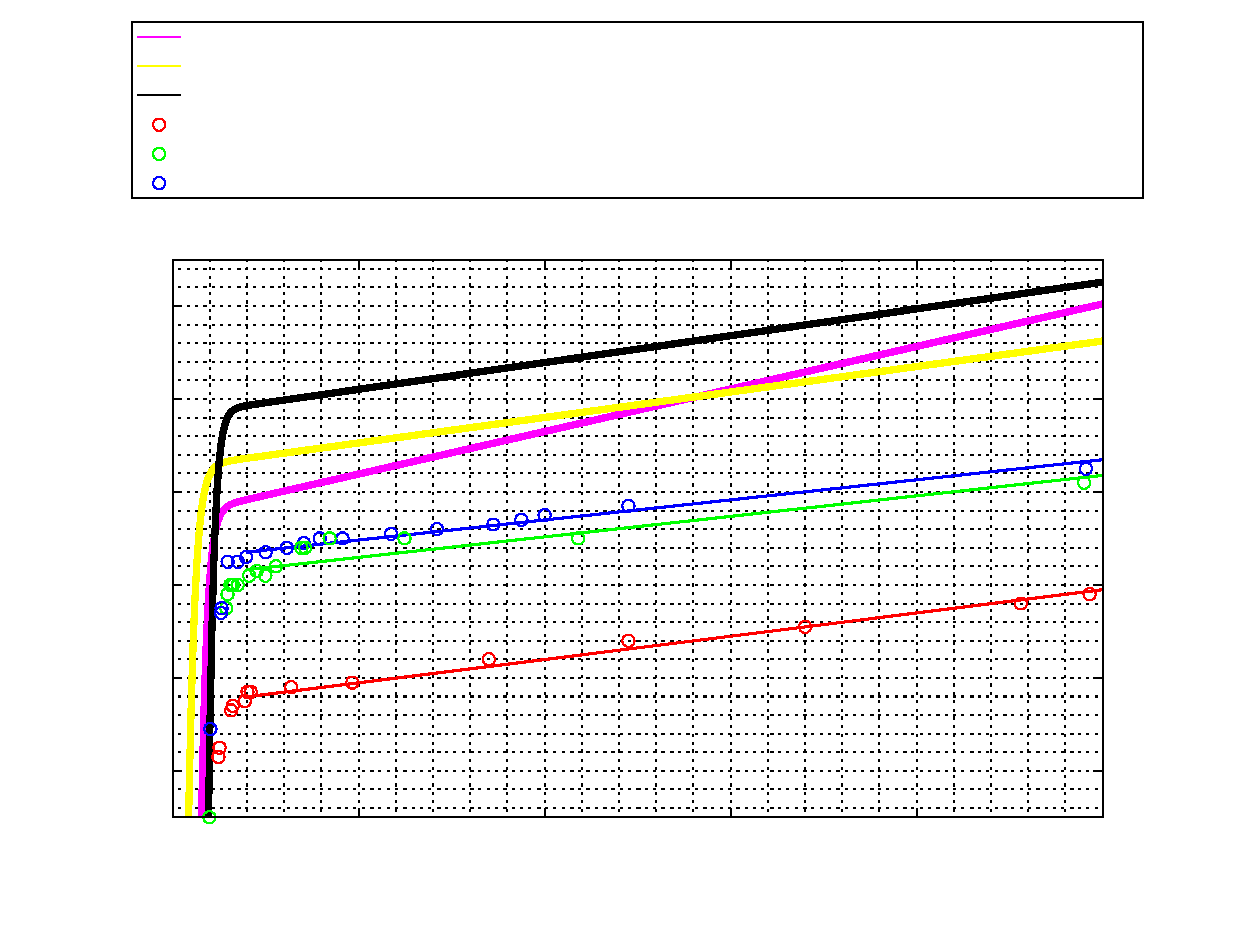
\includegraphics{IcvsVce_5mA-inc}
\end{picture}%
\begin{picture}(576,432)(0,0)
\fontsize{10}{0}
\selectfont\put(74.88,42.5251){\makebox(0,0)[t]{\textcolor[rgb]{0,0,0}{{0}}}}
\fontsize{10}{0}
\selectfont\put(164.16,42.5251){\makebox(0,0)[t]{\textcolor[rgb]{0,0,0}{{1000}}}}
\fontsize{10}{0}
\selectfont\put(253.44,42.5251){\makebox(0,0)[t]{\textcolor[rgb]{0,0,0}{{2000}}}}
\fontsize{10}{0}
\selectfont\put(342.72,42.5251){\makebox(0,0)[t]{\textcolor[rgb]{0,0,0}{{3000}}}}
\fontsize{10}{0}
\selectfont\put(432,42.5251){\makebox(0,0)[t]{\textcolor[rgb]{0,0,0}{{4000}}}}
\fontsize{10}{0}
\selectfont\put(521.28,42.5251){\makebox(0,0)[t]{\textcolor[rgb]{0,0,0}{{5000}}}}
\fontsize{10}{0}
\selectfont\put(69.8755,69.8298){\makebox(0,0)[r]{\textcolor[rgb]{0,0,0}{{4.2}}}}
\fontsize{10}{0}
\selectfont\put(69.8755,114.45){\makebox(0,0)[r]{\textcolor[rgb]{0,0,0}{{4.4}}}}
\fontsize{10}{0}
\selectfont\put(69.8755,159.07){\makebox(0,0)[r]{\textcolor[rgb]{0,0,0}{{4.6}}}}
\fontsize{10}{0}
\selectfont\put(69.8755,203.69){\makebox(0,0)[r]{\textcolor[rgb]{0,0,0}{{4.8}}}}
\fontsize{10}{0}
\selectfont\put(69.8755,248.309){\makebox(0,0)[r]{\textcolor[rgb]{0,0,0}{{5}}}}
\fontsize{10}{0}
\selectfont\put(69.8755,292.929){\makebox(0,0)[r]{\textcolor[rgb]{0,0,0}{{5.2}}}}
\fontsize{10}{0}
\selectfont\put(298.08,31.5251){\makebox(0,0)[t]{\textcolor[rgb]{0,0,0}{{$V_{CE} [\unit{mV}]$}}}}
\fontsize{10}{0}
\selectfont\put(50.8755,181.38){\rotatebox{90}{\makebox(0,0)[b]{\textcolor[rgb]{0,0,0}{{$I_C [\unit{mA}]$}}}}}
\fontsize{10}{0}
\selectfont\put(81.4068,422.224){\makebox(0,0)[l]{\textcolor[rgb]{0,0,0}{{\texttt{PHIL\_BJT} $r_o = 10,91814 \unit{k\Omega}$  $V_A= 51,82703 \unit{V}$ $I_{C_{sat}} = 4,746873 \unit{mA}$}}}}
\fontsize{10}{0}
\selectfont\put(81.4068,408.164){\makebox(0,0)[l]{\textcolor[rgb]{0,0,0}{{\texttt{SIEMENS} $r_o = 18,26616 \unit{k\Omega}$  $V_A= 88,60728\unit{V}$  $I_{C_{sat}} = 4,850897 \unit{mA}$}}}}
\fontsize{10}{0}
\selectfont\put(81.4068,394.104){\makebox(0,0)[l]{\textcolor[rgb]{0,0,0}{{modelo modificado $r_o = 17,34281 \unit{k\Omega}$  $V_A= 90,66048\unit{V}$ $I_{C_{sat}} = 4,963302 \unit{mA}$}}}}
\fontsize{10}{0}
\selectfont\put(81.4068,380.044){\makebox(0,0)[l]{\textcolor[rgb]{0,0,0}{{transistor 1 $r_o = 19,97264 \unit{k\Omega}$  $V_A= 86,67009\unit{V}$ $I_{C_{sat}} = 4,339440 \unit{mA}$}}}}
\fontsize{10}{0}
\selectfont\put(81.4068,365.984){\makebox(0,0)[l]{\textcolor[rgb]{0,0,0}{{transistor 2 $r_o = 22,66700 \unit{k\Omega}$  $V_A= 104,6125\unit{V}$ $I_{C_{sat}} = 4,615188 \unit{mA}$}}}}
\fontsize{10}{0}
\selectfont\put(81.4068,351.924){\makebox(0,0)[l]{\textcolor[rgb]{0,0,0}{{transistor 3 $r_o = 23,13776 \unit{k\Omega}$ $ V_A= 107,6684\unit{V}$ $I_{C_{sat}} = 4,653361 \unit{mA}$}}}}
\end{picture}
\end{document}
